\documentclass{standalone}
\usepackage{tikz}
\usetikzlibrary{patterns, positioning}
\usetikzlibrary{shapes.misc}
\usepackage[outline]{contour}
\contourlength{1.5pt} 


\begin{document}
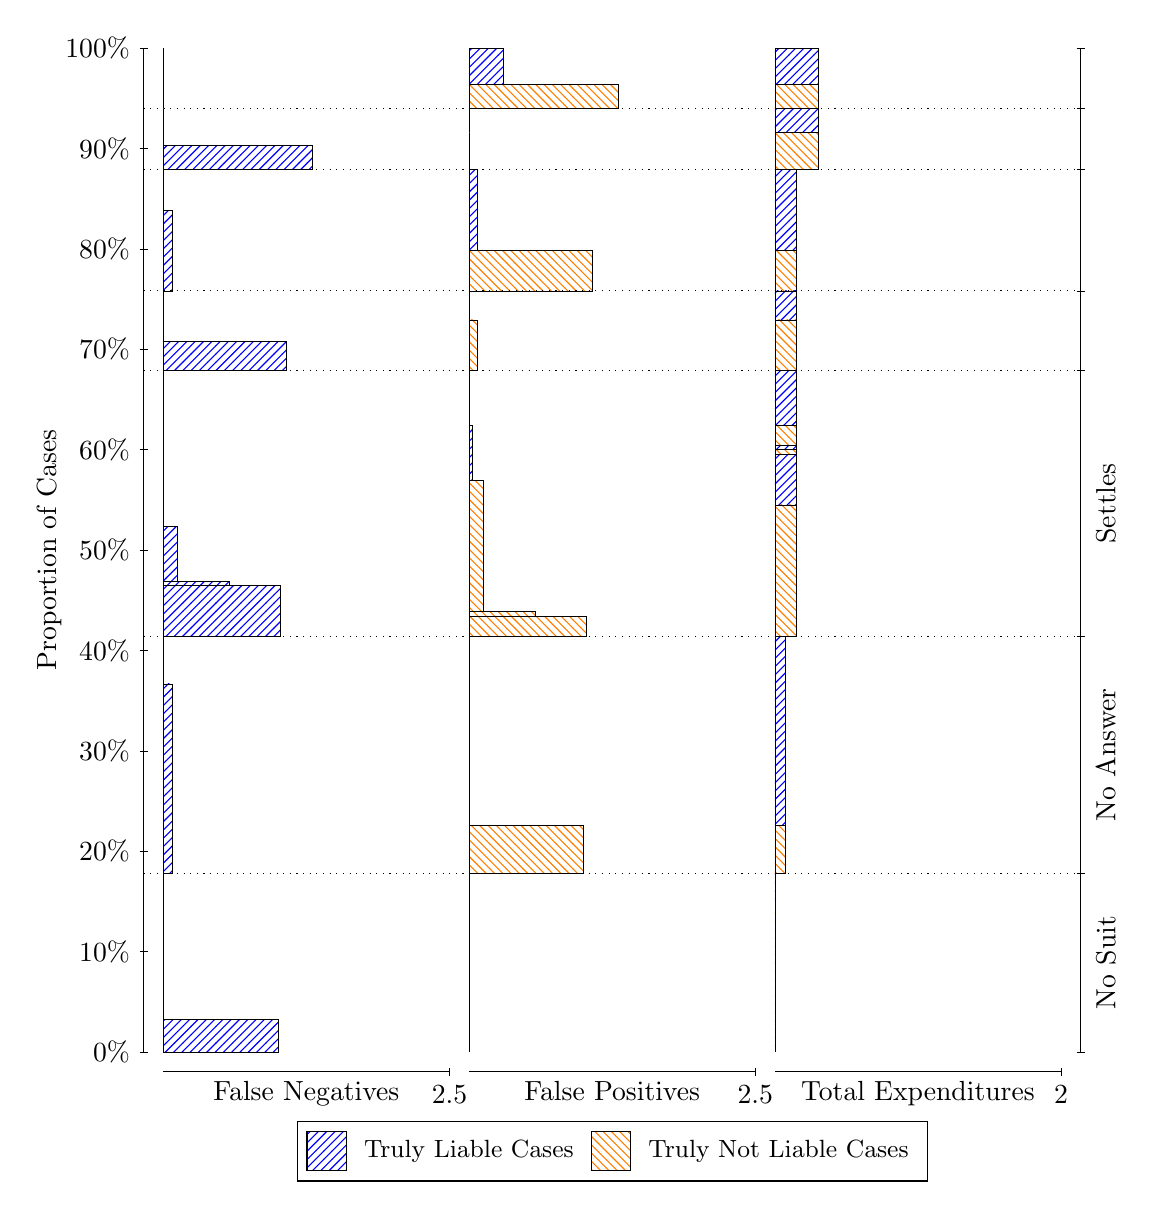
\begin{tikzpicture}
\draw[black, very thin] (1.5,1.75) -- (1.5,14.5);
\node[rotate=90, text=black, anchor=center] at (0.3, 8.125) {Proportion of Cases};
\draw[black, very thin] (1.45,1.75) -- (1.55,1.75);
\node[text=black, anchor=east] at (1.45, 1.75) {0\%};
\draw[black, very thin] (1.45,3.025) -- (1.55,3.025);
\node[text=black, anchor=east] at (1.45, 3.025) {10\%};
\draw[black, very thin] (1.45,4.3) -- (1.55,4.3);
\node[text=black, anchor=east] at (1.45, 4.3) {20\%};
\draw[black, very thin] (1.45,5.575) -- (1.55,5.575);
\node[text=black, anchor=east] at (1.45, 5.575) {30\%};
\draw[black, very thin] (1.45,6.85) -- (1.55,6.85);
\node[text=black, anchor=east] at (1.45, 6.85) {40\%};
\draw[black, very thin] (1.45,8.125) -- (1.55,8.125);
\node[text=black, anchor=east] at (1.45, 8.125) {50\%};
\draw[black, very thin] (1.45,9.4) -- (1.55,9.4);
\node[text=black, anchor=east] at (1.45, 9.4) {60\%};
\draw[black, very thin] (1.45,10.675) -- (1.55,10.675);
\node[text=black, anchor=east] at (1.45, 10.675) {70\%};
\draw[black, very thin] (1.45,11.95) -- (1.55,11.95);
\node[text=black, anchor=east] at (1.45, 11.95) {80\%};
\draw[black, very thin] (1.45,13.225) -- (1.55,13.225);
\node[text=black, anchor=east] at (1.45, 13.225) {90\%};
\draw[black, very thin] (1.45,14.5) -- (1.55,14.5);
\node[text=black, anchor=east] at (1.45, 14.5) {100\%};

\draw[black, very thin] (13.4,1.75) -- (13.4,14.5);
\draw[black, very thin] (13.35,1.75) -- (13.45,1.75);
\node[anchor=west] at (13.35, 1.75) {};
\draw[black, very thin] (13.35,4.0212) -- (13.45,4.0212);
\node[anchor=west] at (13.35, 4.0212) {};
\draw[black, very thin] (13.35,7.0276) -- (13.45,7.0276);
\node[anchor=west] at (13.35, 7.0276) {};
\draw[black, very thin] (13.35,10.407) -- (13.45,10.407);
\node[anchor=west] at (13.35, 10.407) {};
\draw[black, very thin] (13.35,11.416) -- (13.45,11.416);
\node[anchor=west] at (13.35, 11.416) {};
\draw[black, very thin] (13.35,12.958) -- (13.45,12.958);
\node[anchor=west] at (13.35, 12.958) {};
\draw[black, very thin] (13.35,13.735) -- (13.45,13.735);
\node[anchor=west] at (13.35, 13.735) {};
\draw[black, very thin] (13.35,14.5) -- (13.45,14.5);
\node[anchor=west] at (13.35, 14.5) {};

\draw[black, very thin, pattern color=blue, pattern=north east lines] (1.75,1.75) rectangle (3.2033,2.1651);
\draw[black, very thin, pattern color=orange, pattern=north west lines] (1.75,2.1651) rectangle (1.75,4.0212);
\draw[black, very thin, pattern color=blue, pattern=north east lines] (1.75,4.0212) rectangle (1.859,6.4258);
\draw[black, very thin, pattern color=orange, pattern=north west lines] (1.75,6.4258) rectangle (1.75,7.0276);
\draw[black, very thin, pattern color=blue, pattern=north east lines] (1.75,7.0276) rectangle (3.2397,7.6731);
\draw[black, very thin, pattern color=blue, pattern=north east lines] (1.75,7.6731) rectangle (2.5857,7.7296);
\draw[black, very thin, pattern color=blue, pattern=north east lines] (1.75,7.7296) rectangle (1.9317,8.4235);
\draw[black, very thin, pattern color=orange, pattern=north west lines] (1.75,8.4235) rectangle (1.75,10.407);
\draw[black, very thin, pattern color=blue, pattern=north east lines] (1.75,10.407) rectangle (3.3123,10.775);
\draw[black, very thin, pattern color=orange, pattern=north west lines] (1.75,10.775) rectangle (1.75,11.416);
\draw[black, very thin, pattern color=blue, pattern=north east lines] (1.75,11.416) rectangle (1.859,12.44);
\draw[black, very thin, pattern color=orange, pattern=north west lines] (1.75,12.44) rectangle (1.75,12.958);
\draw[black, very thin, pattern color=blue, pattern=north east lines] (1.75,12.958) rectangle (3.6393,13.266);
\draw[black, very thin, pattern color=orange, pattern=north west lines] (1.75,13.266) rectangle (1.75,13.735);
\draw[black, very thin, pattern color=orange, pattern=north west lines] (1.75,13.735) rectangle (1.75,14.041);
\draw[black, very thin, pattern color=blue, pattern=north east lines] (1.75,14.041) rectangle (1.75,14.5);
\draw[black, very thin, pattern color=orange, pattern=north west lines] (5.6333,1.75) rectangle (5.6333,3.606);
\draw[black, very thin, pattern color=blue, pattern=north east lines] (5.6333,3.606) rectangle (5.6333,4.0212);
\draw[black, very thin, pattern color=orange, pattern=north west lines] (5.6333,4.0212) rectangle (7.0867,4.6229);
\draw[black, very thin, pattern color=blue, pattern=north east lines] (5.6333,4.6229) rectangle (5.6333,7.0276);
\draw[black, very thin, pattern color=orange, pattern=north west lines] (5.6333,7.0276) rectangle (7.123,7.2853);
\draw[black, very thin, pattern color=orange, pattern=north west lines] (5.6333,7.2853) rectangle (6.469,7.3417);
\draw[black, very thin, pattern color=orange, pattern=north west lines] (5.6333,7.3417) rectangle (5.815,9.0113);
\draw[black, very thin, pattern color=blue, pattern=north east lines] (5.6333,9.0113) rectangle (5.6697,9.7052);
\draw[black, very thin, pattern color=blue, pattern=north east lines] (5.6333,9.7052) rectangle (5.6333,10.407);
\draw[black, very thin, pattern color=orange, pattern=north west lines] (5.6333,10.407) rectangle (5.7423,11.048);
\draw[black, very thin, pattern color=blue, pattern=north east lines] (5.6333,11.048) rectangle (5.6333,11.416);
\draw[black, very thin, pattern color=orange, pattern=north west lines] (5.6333,11.416) rectangle (7.1957,11.934);
\draw[black, very thin, pattern color=blue, pattern=north east lines] (5.6333,11.934) rectangle (5.7423,12.958);
\draw[black, very thin, pattern color=orange, pattern=north west lines] (5.6333,12.958) rectangle (5.6333,13.428);
\draw[black, very thin, pattern color=blue, pattern=north east lines] (5.6333,13.428) rectangle (5.6333,13.735);
\draw[black, very thin, pattern color=orange, pattern=north west lines] (5.6333,13.735) rectangle (7.5227,14.041);
\draw[black, very thin, pattern color=blue, pattern=north east lines] (5.6333,14.041) rectangle (6.0693,14.5);
\draw[black, very thin, pattern color=orange, pattern=north west lines] (9.5167,1.75) rectangle (9.5167,3.606);
\draw[black, very thin, pattern color=blue, pattern=north east lines] (9.5167,3.606) rectangle (9.5167,4.0212);
\draw[black, very thin, pattern color=orange, pattern=north west lines] (9.5167,4.0212) rectangle (9.6529,4.6229);
\draw[black, very thin, pattern color=blue, pattern=north east lines] (9.5167,4.6229) rectangle (9.6529,7.0276);
\draw[black, very thin, pattern color=orange, pattern=north west lines] (9.5167,7.0276) rectangle (9.7892,8.6971);
\draw[black, very thin, pattern color=blue, pattern=north east lines] (9.5167,8.6971) rectangle (9.7892,9.3427);
\draw[black, very thin, pattern color=orange, pattern=north west lines] (9.5167,9.3427) rectangle (9.7892,9.3992);
\draw[black, very thin, pattern color=blue, pattern=north east lines] (9.5167,9.3992) rectangle (9.7892,9.4557);
\draw[black, very thin, pattern color=orange, pattern=north west lines] (9.5167,9.4557) rectangle (9.7892,9.7134);
\draw[black, very thin, pattern color=blue, pattern=north east lines] (9.5167,9.7134) rectangle (9.7892,10.407);
\draw[black, very thin, pattern color=orange, pattern=north west lines] (9.5167,10.407) rectangle (9.7892,11.048);
\draw[black, very thin, pattern color=blue, pattern=north east lines] (9.5167,11.048) rectangle (9.7892,11.416);
\draw[black, very thin, pattern color=orange, pattern=north west lines] (9.5167,11.416) rectangle (9.7892,11.934);
\draw[black, very thin, pattern color=blue, pattern=north east lines] (9.5167,11.934) rectangle (9.7892,12.958);
\draw[black, very thin, pattern color=orange, pattern=north west lines] (9.5167,12.958) rectangle (10.062,13.428);
\draw[black, very thin, pattern color=blue, pattern=north east lines] (9.5167,13.428) rectangle (10.062,13.735);
\draw[black, very thin, pattern color=orange, pattern=north west lines] (9.5167,13.735) rectangle (10.062,14.041);
\draw[black, very thin, pattern color=blue, pattern=north east lines] (9.5167,14.041) rectangle (10.062,14.5);
\draw[black, dotted] (1.5,4.0212) -- (13.4,4.0212);
\draw[black, dotted] (1.5,7.0276) -- (13.4,7.0276);
\draw[black, dotted] (1.5,10.407) -- (13.4,10.407);
\draw[black, dotted] (1.5,11.416) -- (13.4,11.416);
\draw[black, dotted] (1.5,12.958) -- (13.4,12.958);
\draw[black, dotted] (1.5,13.735) -- (13.4,13.735);
\draw[black, very thin] (1.75,1.5) -- (5.3833,1.5);
\node[text=black, anchor=north] at (3.5667, 1.5) {False Negatives};
\draw[black, very thin] (5.3833,1.45) -- (5.3833,1.55);
\node[text=black, anchor=north] at (5.3833, 1.45) {2.5};

\draw[black, very thin] (5.6333,1.5) -- (9.2667,1.5);
\node[text=black, anchor=north] at (7.45, 1.5) {False Positives};
\draw[black, very thin] (9.2667,1.45) -- (9.2667,1.55);
\node[text=black, anchor=north] at (9.2667, 1.45) {2.5};

\draw[black, very thin] (9.5167,1.5) -- (13.15,1.5);
\node[text=black, anchor=north] at (11.333, 1.5) {Total Expenditures};
\draw[black, very thin] (13.15,1.45) -- (13.15,1.55);
\node[text=black, anchor=north] at (13.15, 1.45) {2};

\node[text=black, centered, rotate=90] at (13.72, 2.8856) {\contour{white}{No Suit}};
\node[text=black, centered, rotate=90] at (13.72, 5.5244) {\contour{white}{No Answer}};
\node[text=black, centered, rotate=90] at (13.72, 8.7174) {\contour{white}{Settles}};





\draw (7.449999999999999,1.5) node[draw=none] (baseCoordinate) {};
\begin{scope}[align=center]
        \matrix[scale=0.5, draw=black, below=0.5cm of baseCoordinate, nodes={draw}, column sep=0.1cm]{
            \node[rectangle, draw, minimum width=0.5cm, minimum height=0.5cm, pattern color=blue, pattern=north east lines] {}; &
            \node[draw=none, font=\small, text=black] (B) {Truly Liable Cases}; &
            \node[rectangle, draw, minimum width=0.5cm, minimum height=0.5cm, pattern color=orange, pattern=north west lines] {}; &
            \node[draw=none, font=\small, text=black] (B) {Truly Not Liable Cases}; \\
            };
\end{scope}

\end{tikzpicture}
\end{document}